\clearpage 
\newpage

%\section*{Figure legends}

\begin{center}
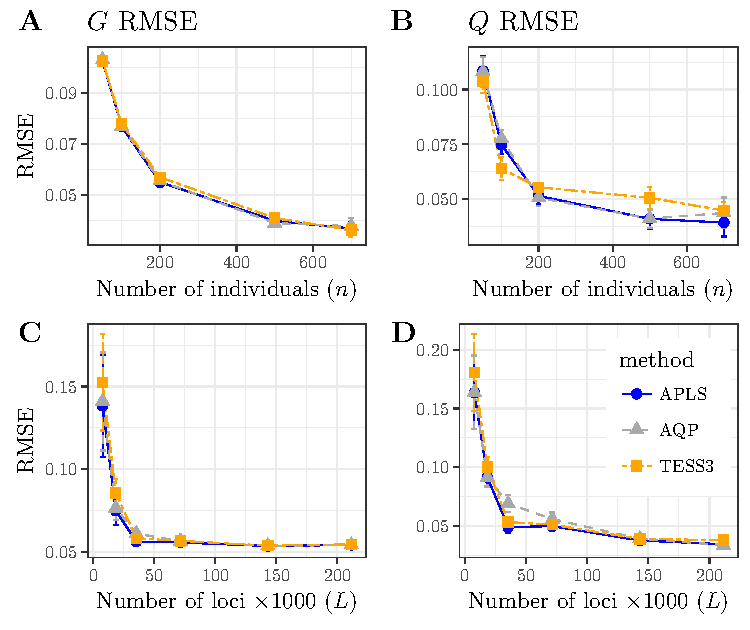
\includegraphics[width=\textwidth]{../Figure1/Figures/figure1.pdf}
\end{center}  
\noindent{\bf Figure 1.} {\bf Root Mean Squared Errors (RMSEs) for the $Q$ and $G$ matrix estimates.} Simulations of spatially admixed populations. A-B) Statistical errors for APLS, AQP and {\tt tess3} estimates as a function of the sample size, $n$ ($L \sim 10^4$). C-D) Statistical errors for APLS, AQP and {\tt tess3} estimates as a function of the number of loci, $L$ ($n = 200$).

\clearpage 
\newpage


\begin{center}
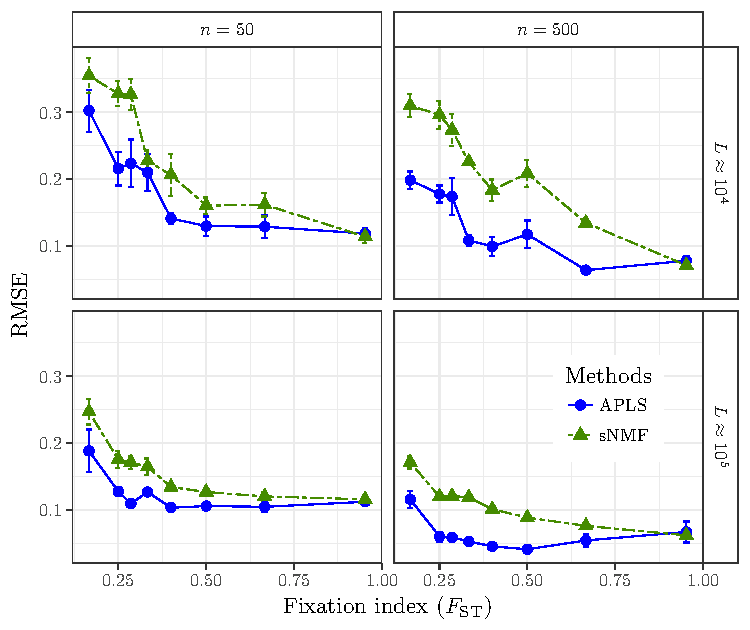
\includegraphics[width=\textwidth]{../Figure2/Figures/figure2.pdf}
\end{center}  
\noindent{\bf Figure 2.} {\bf Root Mean Squared Errors (RMSEs) for the $Q$ estimates.} Simulations of spatially admixed populations for several values of fixation index ($F_{\rm ST}$) between ancestral populations. Ancestral populations are simulated with Wright's two-island models and the fixation index is defined as $1 / (1 + 4 N_0 m)$ where $m$ is the migration rate and $N_0$ the effective population size. The statistical errors for sNMF and APLS are represented as a function of $F_{\rm ST}$. 

\clearpage 
\newpage

\begin{center}
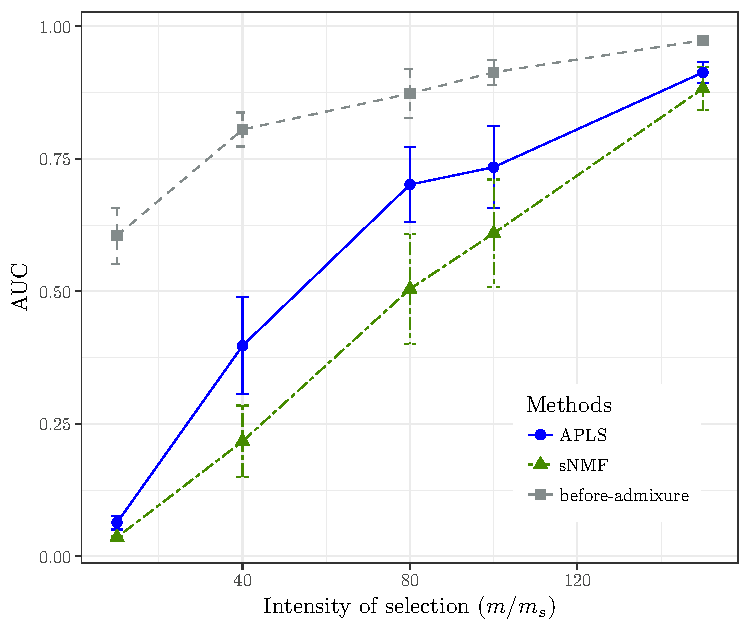
\includegraphics[width=\textwidth]{../Figure3/Figures/figure3.pdf}
\end{center}
\noindent{\bf Figure 3.} {\bf Area under the precision-recall curve (AUC)}. Neutrality tests applied to simulations of spatially admixed populations. AUCs for tests based on $F_{\rm ST}$ with the true ancestral populations,  spatial ancestry estimates computed with APLS algorithms, non-spatial ({\tt structure}-like) ancestry estimates computed with the {\tt snmf} algorithm. The relative intensity of selection in ancestral populations, defined as the ratio $m/m_s$, was varied in the range $1-160$.


\clearpage 
\newpage

\begin{center}
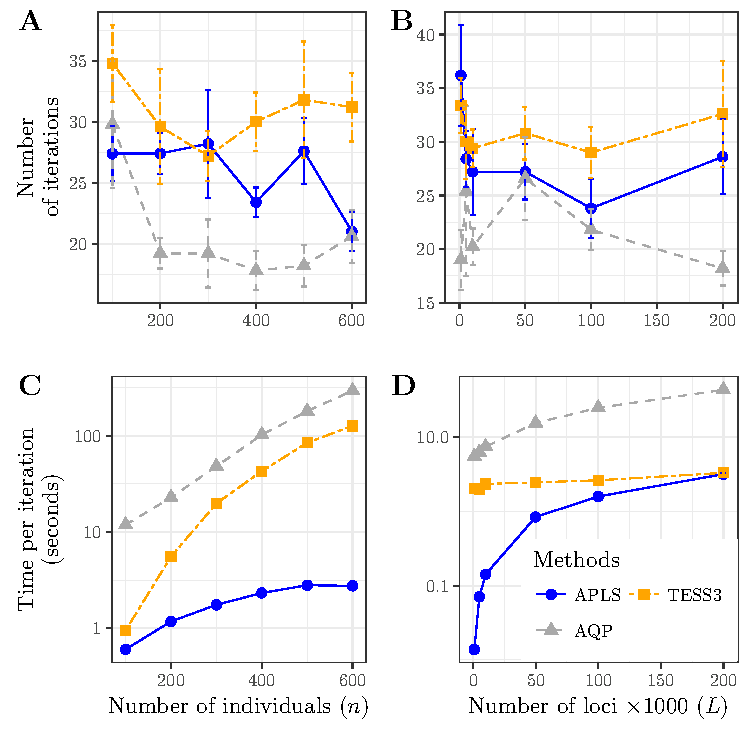
\includegraphics[width=\textwidth]{../Figure4/Figures/figure4.pdf}
\end{center}
\noindent{\bf Figure 4.} {\bf Number of iterations and runtimes for the AQP, APLS and {\tt tess3} algorithm implementations}. A-B)   Total number of iterations before an algorithm reached a steady solution. C-D) Runtime for a single iteration (seconds). The number of SNPs was kept fixed to $L = 50$k in A and C. The number of individuals was kept fixed to $n = 150$ in B and D.


\clearpage 
\newpage

\begin{center}
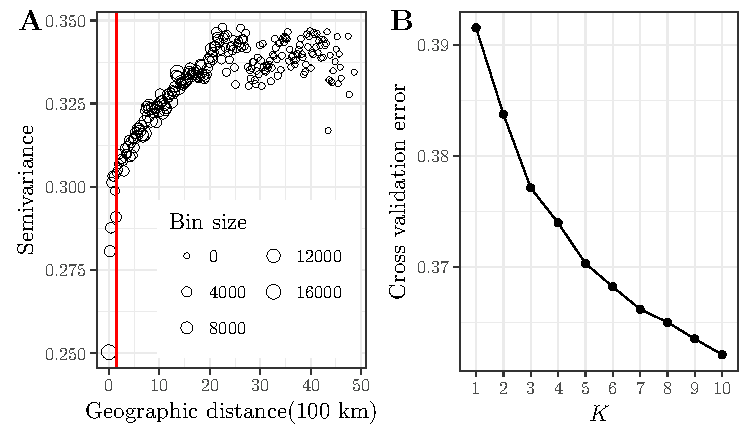
\includegraphics[width=\textwidth]{../Figure5/Figures/figure5.pdf}
\end{center}
\noindent{\bf Figure 5.} {\bf Range $\sigma$ and choice of $K$ for the APLS algorithm}. A) Empirical variogram for the {\it A. thaliana} data. The red vertical line shows the range value $\sigma = 1.5$. B) Cross validation error as function of the number of ancestral populations, $K$.

\clearpage 
\newpage

\begin{center}
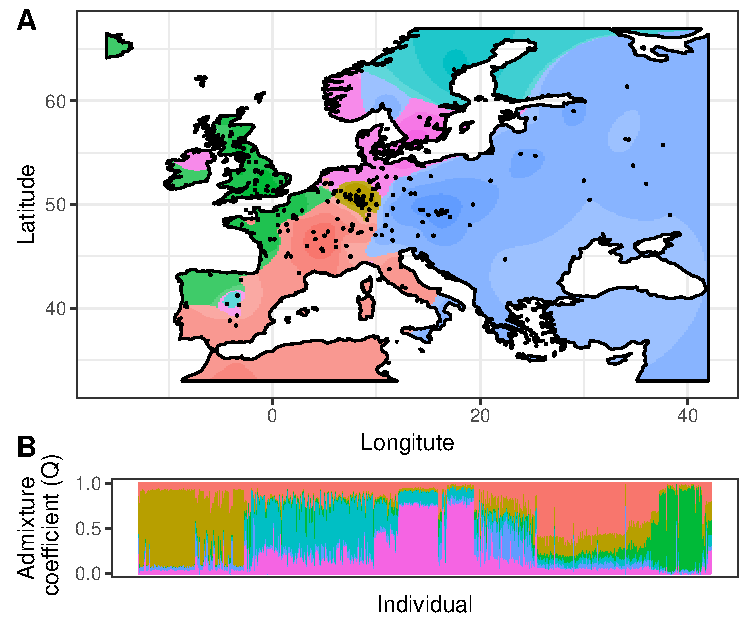
\includegraphics[width=\textwidth]{../Figure5/Figures/map.pdf}
\end{center}
\noindent{\bf Figure 6.} {\bf {\it A. thaliana} ancestry coeficients}. Ancestry coefficient estimates computed by the APLS algorithm with $K=6$ ancestral populations and $\sigma = 1.5$ for the range parameter. A) Geographic map of ancestry coefficients. B) Barplot of ancestry coefficients.

\clearpage 
\newpage

\begin{center}
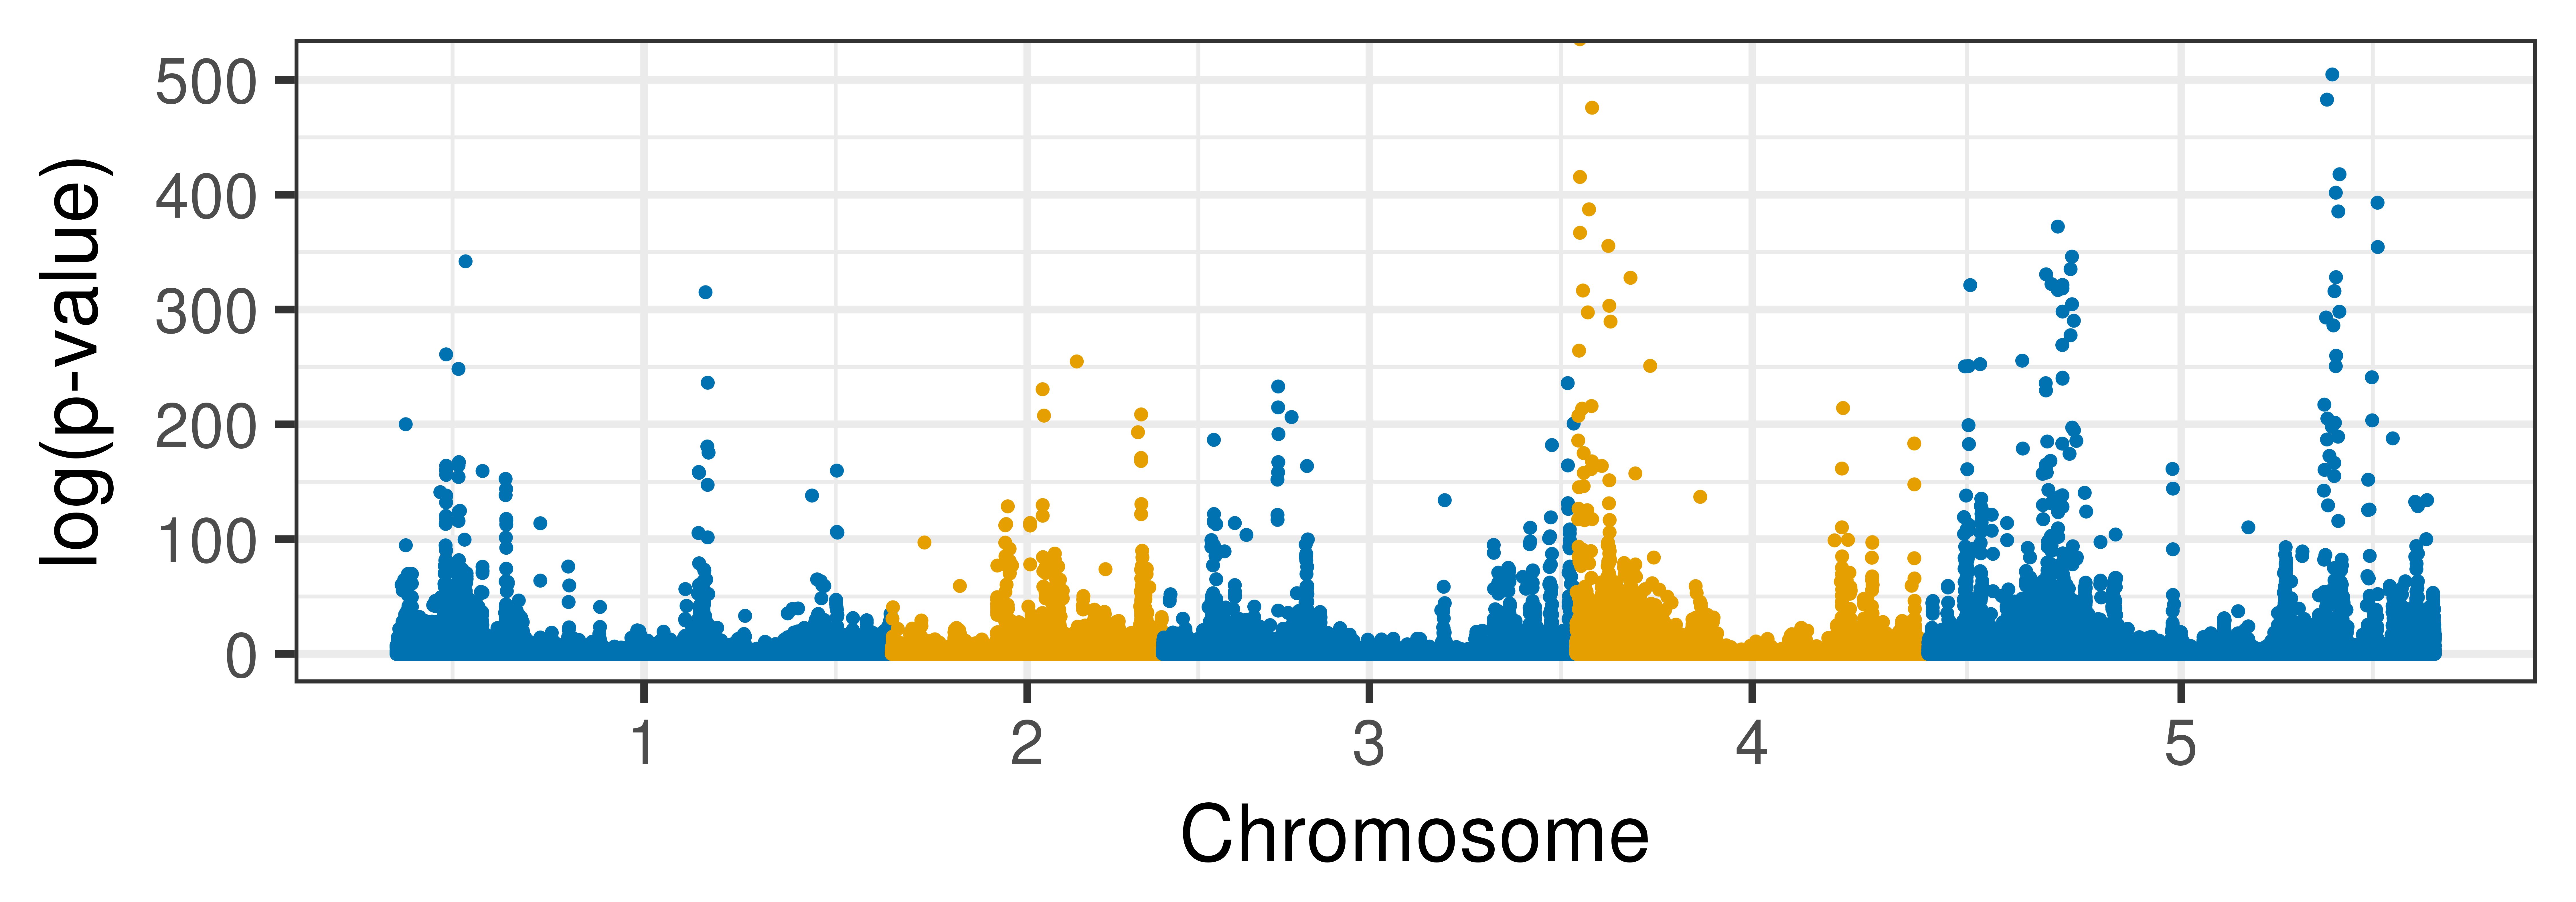
\includegraphics[width=0.60\paperwidth]{../Figure5/Figures/manhattanplot.png}
%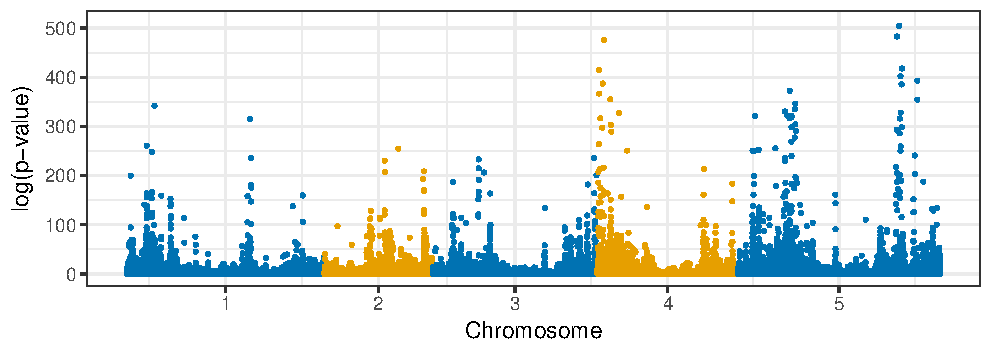
\includegraphics[width=\textwidth]{../Figure5/Figures/manhattanplot.pdf}
\end{center}
\noindent{\bf Figure 7.} {\bf Local adaptation in European lines of \bf {\it A.  thaliana} }. Manhattan plot of $-\log(p$\rm -value$)$.  $p$-value were computed from population structure estimated by the APLS algorithm with $K=6$ ancestral populations and $\sigma = 1.5$ for the range parameter.

%\includegraphics[width=12cm]{Figures/Figure_2.pdf}
%\noindent{\bf Figure 2.} {\bf .} 


